\documentclass[a4paper,12pt]{report}
\usepackage[T2A]{fontenc}
\usepackage[utf8]{inputenc}
\usepackage[english,russian]{babel}
\usepackage{graphicx}
\usepackage{wrapfig}
\usepackage{mathtext} 				% русские буквы в фомулах
\usepackage{amsmath,amsfonts,amssymb,amsthm,mathtools} % AMS
\usepackage{icomma} % "Умная" запятая: $0,2$ --- число, $0, 2$ --- перечисление
\usepackage{capt-of}
\usepackage{appendix}
\usepackage{multirow}
\usepackage{hyperref}
\usepackage{floatrow}
\usepackage[left=2cm,right=2cm,
    top=2cm,bottom=2cm,bindingoffset=0cm]{geometry}
\usepackage{multicol} % Несколько колонок
\usepackage{gensymb}
\title{Отчёт по лабораторной работе №4.4.1 

Амплитудная дифракционная решётка.}
\author{Плюскова Н.А. Б04-004 }
\date{\today}

\begin{document}

\maketitle

\section*{1. Аннотация}

В работе требовалось отъюстировать гониометр, исследовать
спектр ртутной лампы, определить период и спектральные характеристики решётки.

\section*{2. Теоретические сведения}

Амплитудную решётку можно представить в виде непрозрачного экрана, в котором прорезано большое число $N$ параллельных щелей — штрихов. Постоянство расстояний между штрихами $d$ (период решётки, или шаг решётки) и шириной штриха $b$ должно выдерживаться с большой точностью.

\begin{center}
    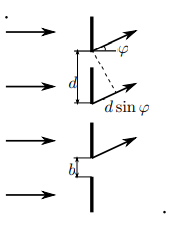
\includegraphics[scale = 1]{pic1.PNG}
    \captionof{figure}{Дифракция
световой волны на
амплитудной решётке}
\end{center}

Наблюдение изображения спектра проводится с помощью зрительной трубы, настроенной на бесконечность (дифракции Фраунгофера на штрихах решётки). В этом случае амплитуда и интенсивность поля световой волны определяются углом $\varphi$ между нормалью к решётке и направлением дифрагировавших лучей. Будем считать, что амплитуды всех интерферирующих волн одинаковы, т.е. фиксирована амплитуда падающей волны и постоянна площадь всех штрихов. Интенсивность дифрагированного света максимальна для углов $\varphi_{m}$, при которых волны, приходящие в точку наблюдения от всех щелей, оказываются в фазе:
\begin{equation}
    d\sin{\varphi_{m}} = m\lambda.
\end{equation}

Рассмотрим пример с двумя спектральными линиями красной и фиолетовой $(\lambda_{red}> \lambda_{purp})$. Для малых углов дифракции угловое расстояние между порядками $\varphi_{m+1} - \varphi \approx \lambda /d$ пропорционально длине волны, поэтому фиолетовые линии следуют чаще чем красные. При m = 5 для красной и m = 6 для фиолетовой они совпадут. 

Некоторые формулы:

\begin{itemize}
    \item Разрешающая способность характеризует возможность прибора различать две близкие спектральные линии с длинами волн $\lambda$ и $\lambda + \delta \lambda$.
    \begin{equation}
        R = \frac{\lambda}{\delta \lambda}
    \end{equation}

    \item Угловая дисперсия - производная зависимости угла отклонения $\varphi(\lambda)$ волны диспергирующим элементом по $\lambda$. По величине угловой дисперсии можно определить угловое расстояние между двумя близкими спектральными линиями: $\delta \varphi \approx D \delta \lambda$:

    \begin{equation}
        D = \frac{d \varphi}{d \lambda} = \frac{m}{d \cdot \cos{\varphi_m}} = \frac{m}{\sqrt{d^2 - m^2 \lambda^2}}
    \end{equation}

    \item Угловое расстояние между линиями определяется:
    \begin{equation}
        \Delta \varphi \approx D \delta \lambda
    \end{equation}

    \item Полуширина линии:
    \begin{equation}
        \delta \varphi = \frac{\lambda}{Nd \cos{\varphi_m}}
    \end{equation}

    \item Дисперсионная область – предельная ширина спектального интервала $\Delta \lambda$ прибора, для которой дифракционные максимумы соседних порядков не перекрываются. Она определяет диапазон длин волн, при которых прибор может быть использован для анализа спектра.
\end{itemize}

\section*{3. Экспериментальная установка}

Оптические приборы, в которых осуществялется физическое разложение электромагнитного излучения намонозроматические составляющие, называются спектральными. По характеру распределения интенсивности в спектральном разложении спектры могут быть разделены на линейчатые и непрерывные.  
Принципиальная установка изображена на рис.\ref{p1}. Свет от источника $S$ попадает на экран с щелью. Коллиматор формирует близкие к параллельному пучок лучей. После, свет попадает надиспергирующий элемент. Наблюдение производится через трубу, установленну на $\infty$

\begin{figure}[H]
    \begin{center}
        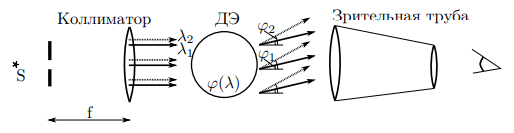
\includegraphics[scale = 1]{pic2.PNG}
        \caption{Схема прибора: источник-коллиматор – диспергирующий элемент – зрительная труба}
    \end{center}
\end{figure}

Каждой монохроматической компоненте с $\lambda$ соответствует один или несколько углов $\varphi(\lambda)$ на выходе из прибора, в направлении которых интенсивность прибора максимальна. При известной зависимости $\varphi(\lambda)$ по измеряемому углу поворота $\varphi$ зрительной трубы можно определить длину волны спектральной линии.  

Наиболее важными характеристиками спектральных приборов являются угловая дисперсия, разрешающая способность и дисперсионная область.
\section*{4. Результаты измерений и обработка данных}

\subsection*{4.1 Определение периода решетки}

Были измерены угловые координаты спектральных линий для $+1$ и $-1$ порядков. Результаты измерений сведем в таблицу 1:

\begin{table}[H]
\centering
\begin{tabular}{|c|cc|c|cc|c|c|}
\hline
\multirow{2}{*}{Цвет} & \multicolumn{2}{c|}{Координата}                  & \multirow{2}{*}{\sigma_{\varphi_{m}}} & \multicolumn{2}{c|}{\multirow{2}{*}{sin\varphi_{m}}} & \multirow{2}{*}{\sigma_{sin \varphi_{m}}} & \multirow{2}{*}{Длина волны $\lambda$, нм} \\ \cline{2-3}
                      & \multicolumn{1}{c|}{-1 порядок} & +1 порядок &                           & \multicolumn{2}{c|}{}                         &                                &                                         \\ \hline
Фиолетовый            & \multicolumn{1}{c|}{$191^{\circ}$ 38' 56''} & $168^{\circ}$ 18' 38'' & \multirow{8}{*}{2,5''}    & \multicolumn{1}{c|}{-0,2019}     & 0,2026     & \multirow{8}{*}{0,0007}        & 404,7                                   \\ \cline{1-3} \cline{5-6} \cline{8-8} 
Синий                 & \multicolumn{1}{c|}{$192^{\circ}$ 33' 09''} & $167^{\circ}$ 21' 53'' &                           & \multicolumn{1}{c|}{-0,2173}     & 0,2187     &                                & 435,8                                   \\ \cline{1-3} \cline{5-6} \cline{8-8} 
Голубой               & \multicolumn{1}{c|}{$194^{\circ}$ 10' 45''} & $165^{\circ}$ 41' 53'' &                           & \multicolumn{1}{c|}{-0,2450}     & 0,2470     &                                & 491,6                                   \\ \cline{1-3} \cline{5-6} \cline{8-8} 
Зеленый               & \multicolumn{1}{c|}{$195^{\circ}$ 46' 30''} & $164^{\circ}$ 03' 51'' &                           & \multicolumn{1}{c|}{-0,2719}     & 0,2746     &                                & 546,1                                   \\ \cline{1-3} \cline{5-6} \cline{8-8} 
Желтый 1              & \multicolumn{1}{c|}{$196^{\circ}$ 41' 11''} & $163^{\circ}$ 07' 49'' &                           & \multicolumn{1}{c|}{-0,2871}     & 0,2902     &                                & 577                                     \\ \cline{1-3} \cline{5-6} \cline{8-8} 
Желтый 2              & \multicolumn{1}{c|}{$196^{\circ}$ 44' 55''} & $163^{\circ}$ 03' 59'' &                           & \multicolumn{1}{c|}{-0,2882}     & 0,2913     &                                & 579,1                                   \\ \cline{1-3} \cline{5-6} \cline{8-8} 
Красный 1             & \multicolumn{1}{c|}{$197^{\circ}$ 44' 02''} & $162^{\circ}$ 03' 06'' &                           & \multicolumn{1}{c|}{-0,3046}     & 0,3082     &                                & 623,4                                   \\ \cline{1-3} \cline{5-6} \cline{8-8} 
Красный 2             & \multicolumn{1}{c|}{$198^{\circ}$ 03' 42''} & $161^{\circ}$ 42' 50'' &                           & \multicolumn{1}{c|}{-0,3100}     & 0,3138     &                                & 690,7                                   \\ \hline
\end{tabular}
\caption{Координаты спектральных линий для $\pm 1$ порядков}
\end{table}
Здесь погрешность измерений гониометра $\varphi_{m}$ бралось из таблицы ГОСТ, погрешность же $sin \varphi_{m}$ определялась следующей формулой:

\begin{equation*}
    \sigma_{sin \varphi_{m}} = |cos\varphi_{m}\cdot \sigma_{\varphi_{m}}|
\end{equation*}

Построим график зависимости $\sin{\varphi_{m}}$ от длины волны:
\begin{center}
    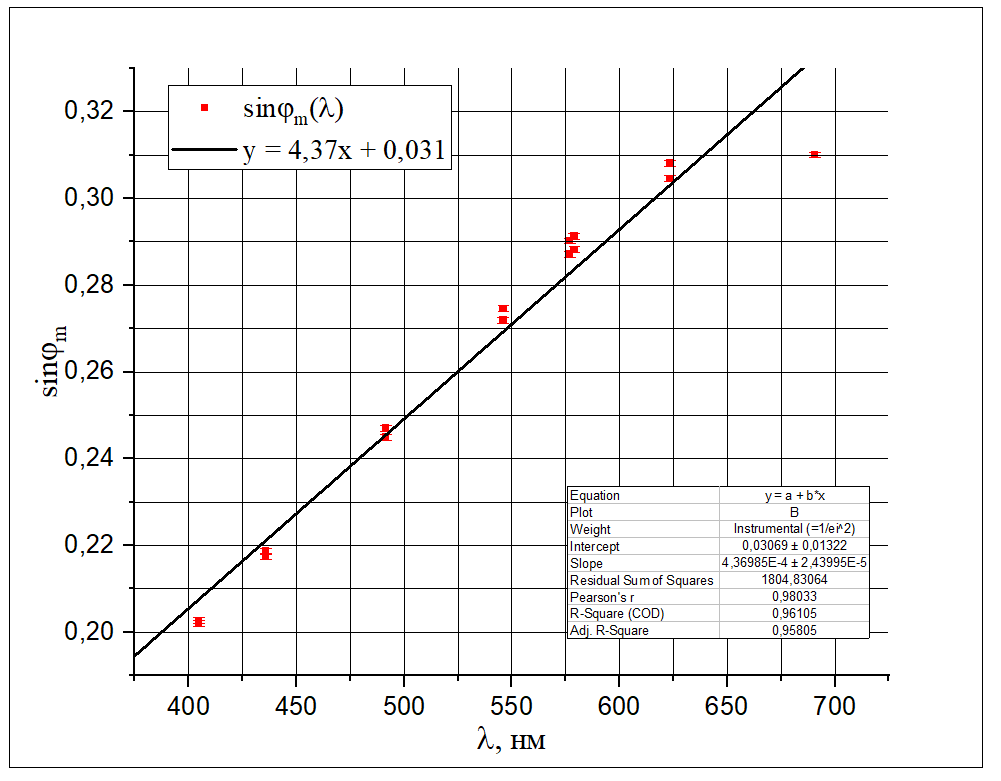
\includegraphics[width = \linewidth]{sin(lambda).png}
    \captionof{figure}{Зависимость $\sin{\varphi_{m}}$ от длины волны}
\end{center}

Найдем коэффициент наклона касательной:
\begin{equation*}
    k = \sqrt{\frac{<xy>-<x>\cdot<y>}{<x^2>-<x>}}
\end{equation*}
\begin{equation*}
    \sigma_k = \sqrt{\frac{1}{n-1}(\frac{<y^2>}{<x^2>}-k^2)}
\end{equation*}
\begin{equation*}
    k = (4,23\pm 0,38) \cdot 10^{-4} \text{ нм}^{-1} 
\end{equation*}

Найдем период дифракционной решетки по формуле (1). Здесь $\varepsilon_{d} = \varepsilon_{k} \approx 9\%$ : 
\begin{equation*}
    d = \frac{\lambda}{\sin{\varphi_{m}}} = \frac{1}{k} = (2,364 \pm 0,213) \text{ мкм}
\end{equation*}

\subsection*{4.2 Определение угловой дисперсии}

Рассчитаем по линиям жёлтого дублета угловую дисперсию в спектрах
разного порядка (формула (3.1)). Построим график зависимости угловой дисперсии от порядка спектра и сравните эту зависимость с расчётной по формуле (3.3) для средней длины волны жёлтого дублета.

Результаты для наглядности представим в таблице: 
\begin{table}[H]
\begin{tabular}{|c|cc|c|c|c|c|c|}
\hline
\multirow{2}{*}{Порядок} & \multicolumn{2}{c|}{Координата}                  & \multirow{2}{*}{\Delta\varphi_{m}} & \multirow{2}{*}{\sigma_{\Delta\varphi_{m}}} & \multirow{2}{*}{$\Delta\lambda$, А} & \multirow{2}{*}{D,\text{рад/А $\cdot 10^{-5}$}} & \multirow{2}{*}{\sigma_{D}, \text{рад/А $\cdot 10^{-5}$}} \\ \cline{2-3}
                         & \multicolumn{1}{c|}{1 линия}      & 2 линия      &                            &                                  &                                    &                    &                          \\ \hline
3                        & \multicolumn{1}{c|}{$117^{\circ}$ 13' 31''} & $116^{\circ}$ 47' 44'' & 0,430^{\circ}                      & \multirow{6}{*}{5''}             & \multirow{6}{*}{2,1}               & 37,1             & 0,5                  \\ \cline{1-4} \cline{7-8} 
2                        & \multicolumn{1}{c|}{$144^{\circ}$ 11' 13''} & $144^{\circ}$ 01' 51'' & 0,156^{\circ}                      &                                  &                                    & 12,9             & 0,5                   \\ \cline{1-4} \cline{7-8} 
1                        & \multicolumn{1}{c|}{$163^{\circ}$ 07' 49''} & $163^{\circ}$ 03' 59'' & 0,064^{\circ}                    &                                  &                                    & 5,3             & 0,5                   \\ \cline{1-4} \cline{7-8} 
-1                       & \multicolumn{1}{c|}{$196^{\circ}$ 41' 11''} & $196^{\circ}$ 44' 55'' & 0,062^{\circ}                      &                                  &                                    &  5,2            & 0,5                   \\ \cline{1-4} \cline{7-8} 
-2                       & \multicolumn{1}{c|}{$214^{\circ}$ 44' 09''} & $214^{\circ}$ 52' 45'' & 0,143^{\circ}                      &                                  &                                    & 11,9             & 0,5                   \\ \cline{1-4} \cline{7-8} 
-3                       & \multicolumn{1}{c|}{$237^{\circ}$ 46' 52''} & $238^{\circ}$ 05' 59'' & 0,319^{\circ}                      &                                  &                                    & 26,5             & 0,5                   \\ \hline
\end{tabular}
\caption{Значения для желтых дуплетов разных порядков }
\end{table}

Отсюда находим средние значения угловой дисперии для разных порядков:
\begin{table}[H]
\begin{tabular}{|l|l|l|l|}
\hline
Порядок                    & 1     & 2     & 3     \\ \hline
$<D>, \text{рад/А} \cdot 10^{-5}$ & $5,24\pm 0,50 $ & $12,45 \pm 0,50$ & $31,79\pm 0,50$ \\ \hline
\end{tabular}
\end{table}

Построим график зависимости угловой дисперсии от порядка спектра: 
\begin{center}
    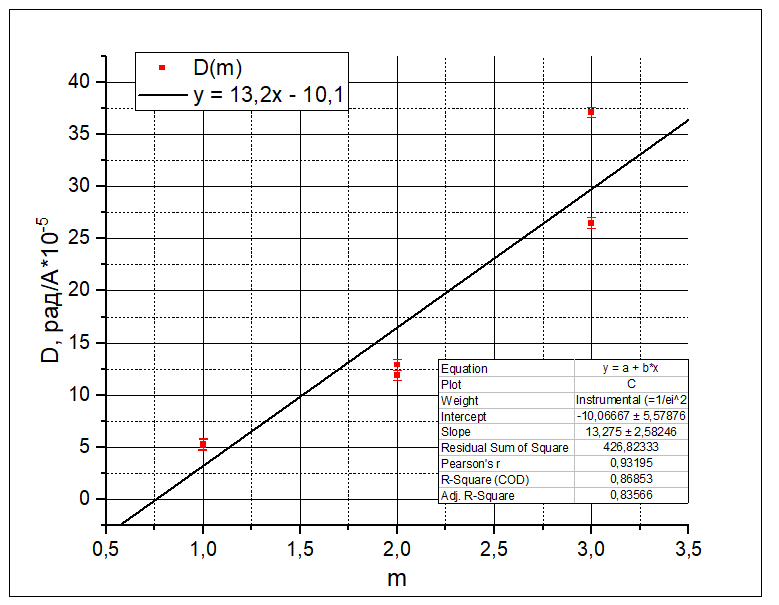
\includegraphics[width = \linewidth]{D(m).png}
    \captionof{figure}{Зависимость угловой дисперсии от порядка спектра, найденная экспериментально}
\end{center}

Рассчитаем угловую дисперсию по формуле (3.3)
\begin{equation*}
    D = \frac{m}{\sqrt{d^{2}-(m\lambda)^{2}}}
\end{equation*} 

Значения угловой дисперии для разных порядков:

\begin{table}[H]
\begin{tabular}{|l|l|l|l|}
\hline
Порядок & 1      & 2     & 3     \\ \hline
$<D>, \text{рад/А $\cdot 10^{-5}$}$       & $5,03 \pm 0,048$ & $11,71 \pm 0,011$ & $27,51 \pm 0,6$ \\ \hline
\end{tabular}
\end{table}

Важно отметить, что экспериментальное и теоретическое значения сходятся в пределах погрешности.

\subsection*{4.3 Оценка разрешающей способности}

В этом пункте мы измеряли ширину желтых спектральных линий, ниже представим результаты измерений: 

\begin{table}[H]
\begin{tabular}{|c|cc|c|c|c|c|c|c|c|}
\hline
\multirow{2}{*}{Порядок} & \multicolumn{2}{c|}{Координаты концов}           & \multirow{2}{*}{\delta\varphi} & \multirow{2}{*}{\sigma_{\delta\varphi}} & \multirow{2}{*}{Длина волны \lambda, нм} & \multirow{2}{*}{D} & \multirow{2}{*}{\sigma_{D}} & \multirow{2}{*}{R} & \multirow{2}{*}{\sigma_{R}} \\ \cline{2-3}
                         & \multicolumn{1}{c|}{начало}       & конец        &                            &                                  &                                         &                    &                          &                    &                          \\ \hline
3                        & \multicolumn{1}{c|}{116 15' 04''} & 116 17' 20'' & 0,0211                & \multirow{6}{*}{5''}             & \multirow{6}{*}{578}                    & 0,2046             & 0,0007                   & 5601,7             & 0,7                      \\ \cline{1-4} \cline{7-10} 
2                        & \multicolumn{1}{c|}{144 05' 20''} & 144 04' 30'' & 0,0139               &                                  &                                         & 0,0743             & 0,0007                   & 3092,1             & 0,6                      \\ \cline{1-4} \cline{7-10} 
1                        & \multicolumn{1}{c|}{164 04' 01''} & 164 03' 28'' & 0,0092                &                                  &                                         & 0,0304             & 0,0007                   & 1916,9             & 0,6                      \\ \cline{1-4} \cline{7-10} 
-1                       & \multicolumn{1}{c|}{196 45' 21''} & 196 44' 41'' & 0,0111                &                                  &                                         & 0,0296             & 0,0007                   & 1539,8             & 0,4                      \\ \cline{1-4} \cline{7-10} 
-2                       & \multicolumn{1}{c|}{214 53' 22''} & 214 52' 44'' & 0,0106                &                                  &                                         & 0,0683             & 0,0007                   & 3740,0             & 0,9                      \\ \cline{1-4} \cline{7-10} 
-3                       & \multicolumn{1}{c|}{238 06' 32''} & 238 05' 33'' & 0,0164                &                                  &                                         & 0,1517             & 0,0007                   & 5350,1             & 0,8                      \\ \hline
\end{tabular}
\end{table}

\begin{table}[H]
\begin{tabular}{|l|l|l|l|}
\hline
Порядок                    & 1     & 2     & 3     \\ \hline
$<R> $ & $1728,3\pm 0,5$ & $3416,0 \pm 0,8$ & $5475,9 \pm 0,8$ \\ \hline
\end{tabular}
\end{table}


По формуле $R = m \cdot N$ найдем количество эффективно работающих шрихов: 
\begin{itemize}
    \item $N_{1} = 1728$
    \item $N_{2} = 1708$
    \item $N_{3} = 2738$
    
\end{itemize}

\section*{5. Вывод}

В этой работе мы исследовали спектр ртутной лампы, поработали с амплитудной дифракционной решеткой. Был определен период самой решетки, найденное значение $(2,364 \pm 0,213)$ мкм. Также, двумя способы мы рассчитали экспериментальную и теоретическую угловые дисперсии,которые совпадают в пределах погрешности, сведем эти результаты в таблицу ниже для наглядности. Также была оценена разрешающая способность спектрального прибора. 

\begin{table}[H]
\begin{tabular}{|l|l|l|l|}
\hline
Порядок & 1 & 2  & 3 \\ \hline
$<D_{\text{эксп}}>, \text{град/нм}$   & $5,24\pm 0,50$ & $12,45 \pm 0,50$ & $31,79 \pm 0,50$ \\ \hline
$<D_{\text{теор}}>, \text{град/нм}$   & $5,03\pm 0,048$ & $11,71 \pm 0,11$ & $27,51 \pm 0,26$ \\ \hline
\end{tabular}
\end{table}

\end{document}

